\begin{frame}{Mechanisms of action of a monoclonal antibody}
    \begin{block}{Neutralisation of a pathogen ; elimination by phagocytosis}
        \begin{figure}
            \centering
            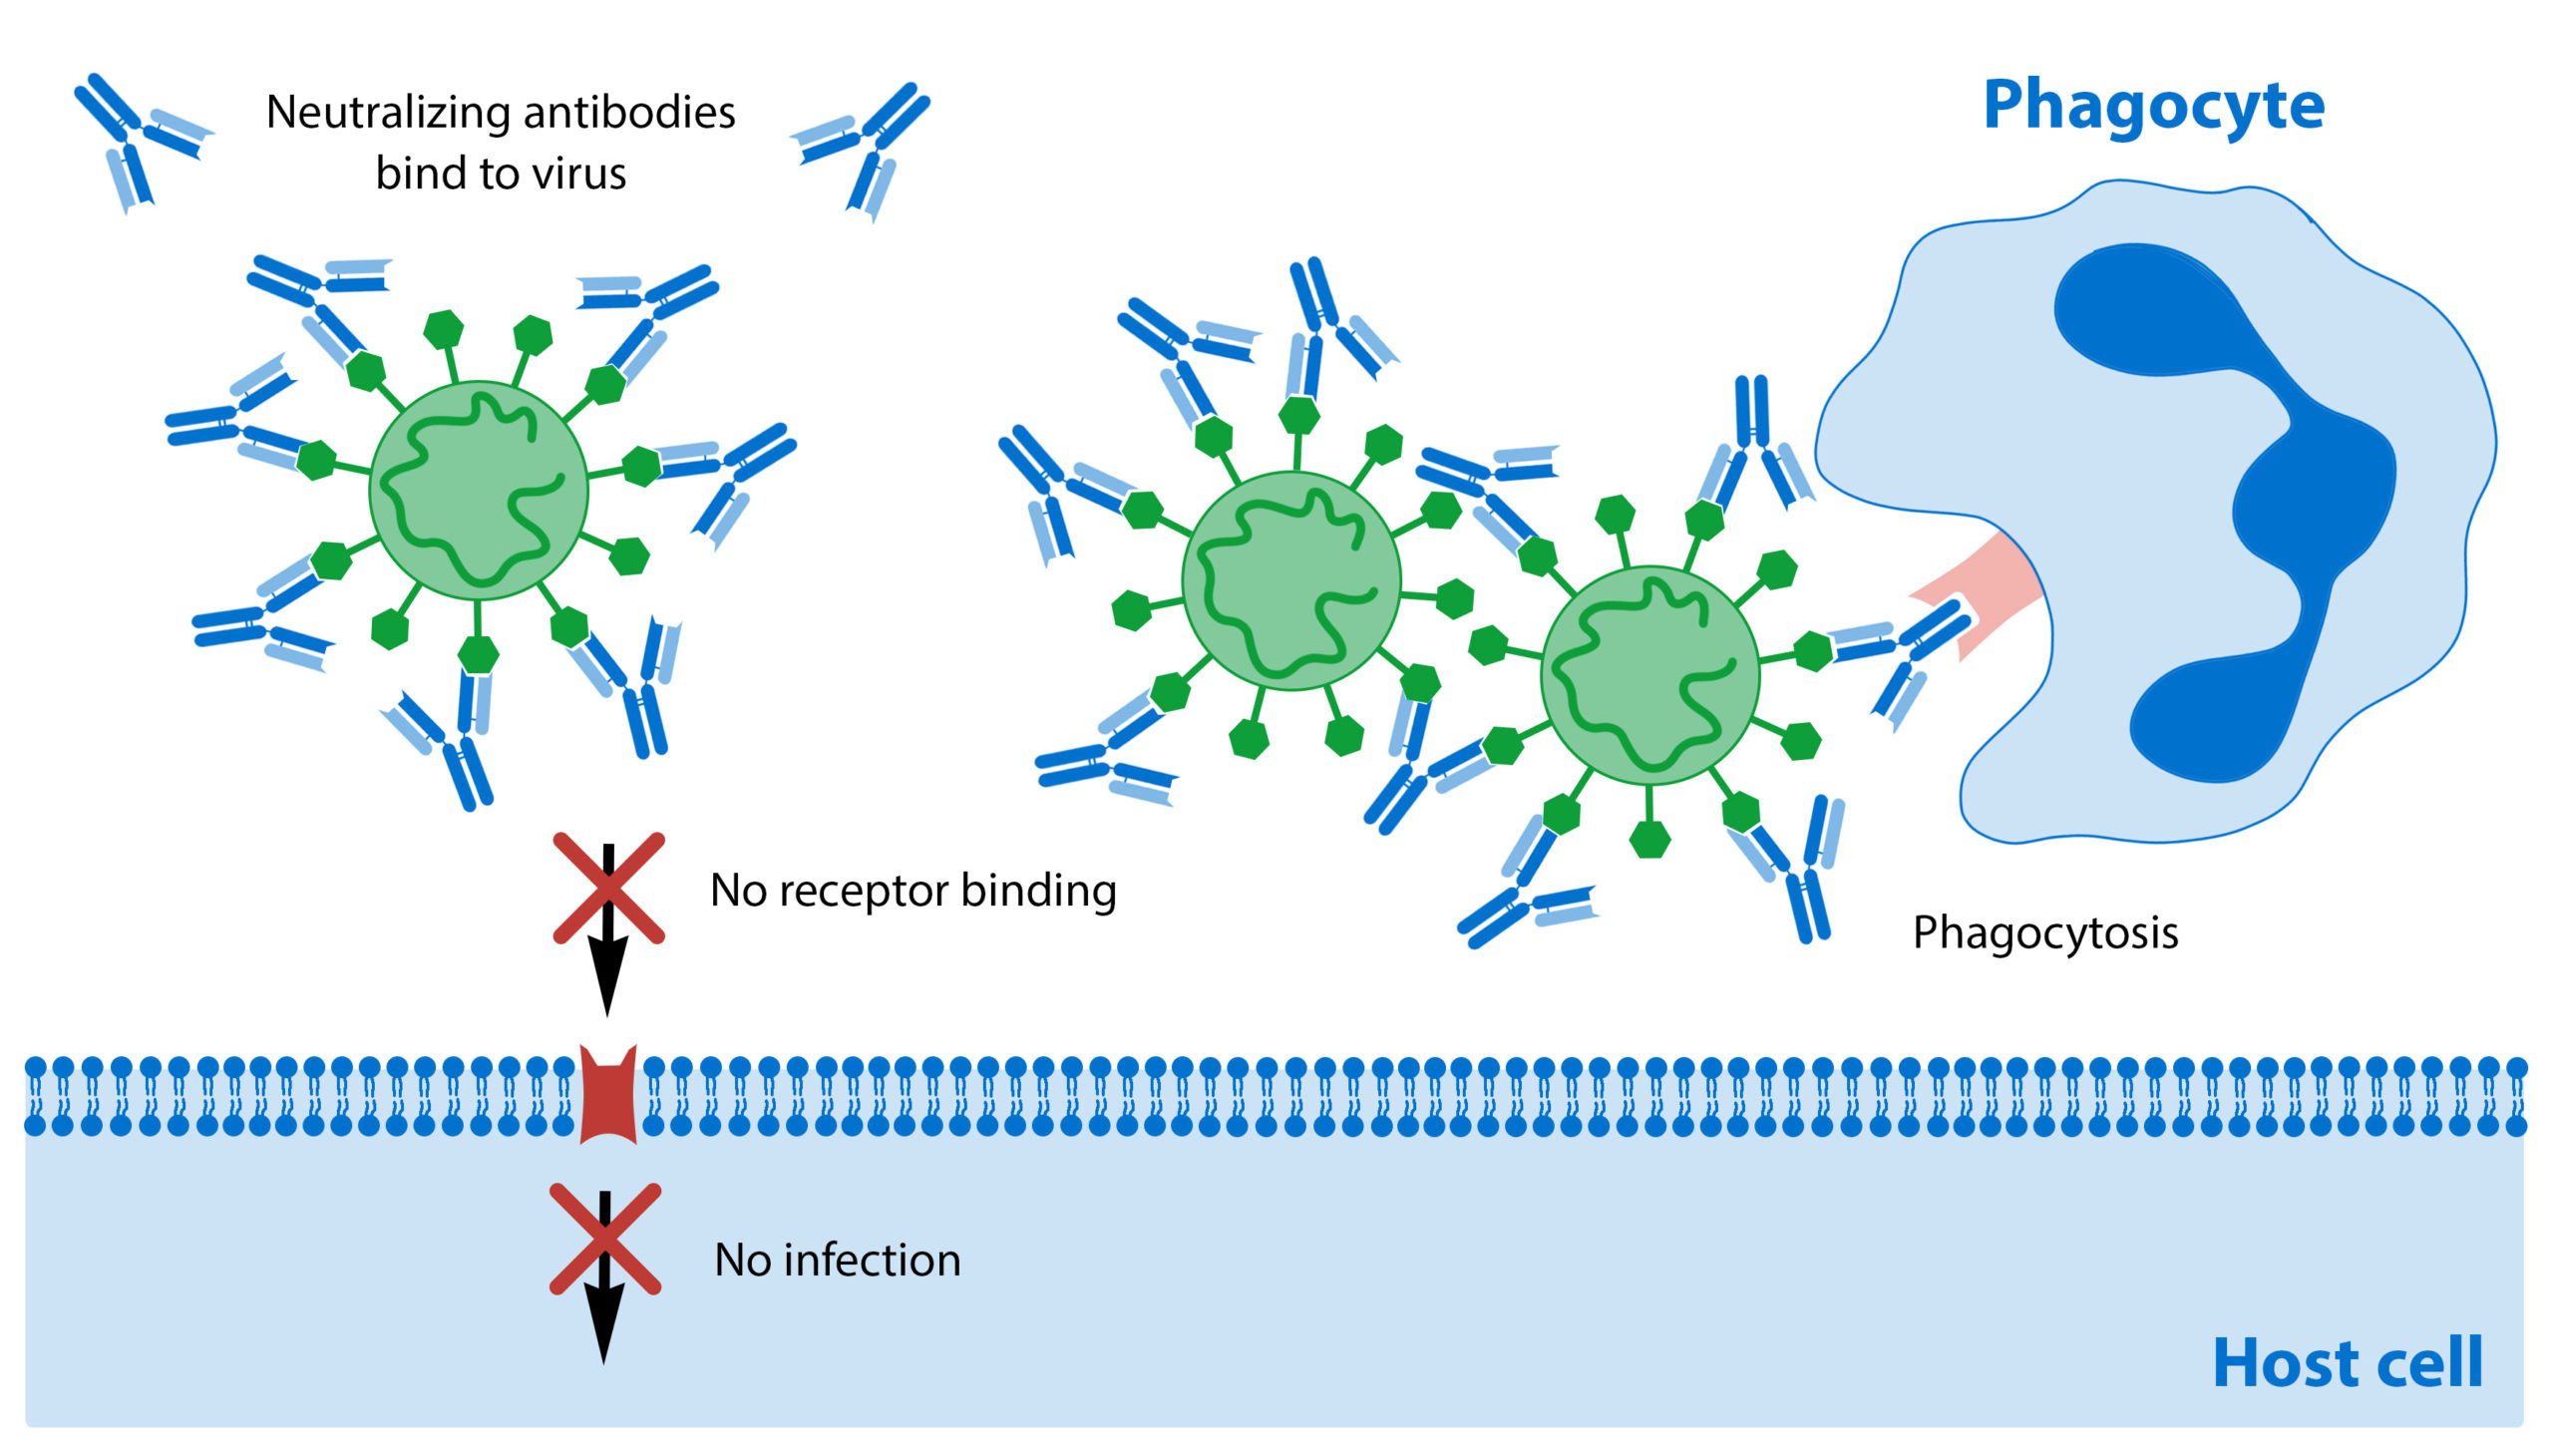
\includegraphics[width=0.9\textwidth]{../Images/antibodies_neutralization.jpeg}
            \caption{Neutralization of a virus by antibodies and cytotoxicity \emph{via} phagocytosis}
            \label{fig:neutralization_antibodies}
        \end{figure}
    \end{block}
\end{frame}

\begin{frame}{Mechanisms of action of a monoclonal antibody}
    \begin{block}{Antibody Dependent Cell Cytotoxicity}
        \begin{figure}
            \centering
            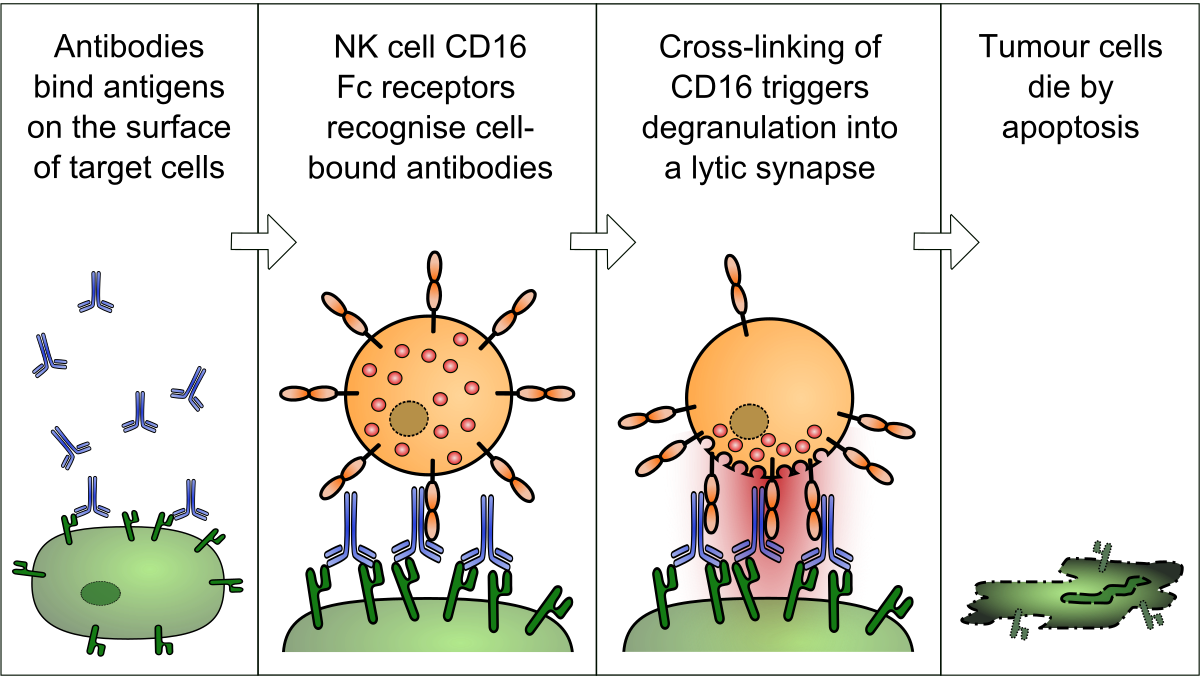
\includegraphics[width=0.8\textwidth]{../Images/Antibody-dependent_Cellular_Cytotoxicity.svg.png}
            \caption{Tumor cell apoptosis induced \emph{via} antibody recognition}
            \label{fig:ADCC}
        \end{figure}
    \end{block}
\end{frame}

\begin{frame}{Mechanisms of action of a monoclonal antibody}
    \begin{block}{Antibody Dependent Cell Cytotoxicity}
        \vspace{1em}
        \begin{minipage}{0.35\textwidth}
            \begin{figure}
                \centering
                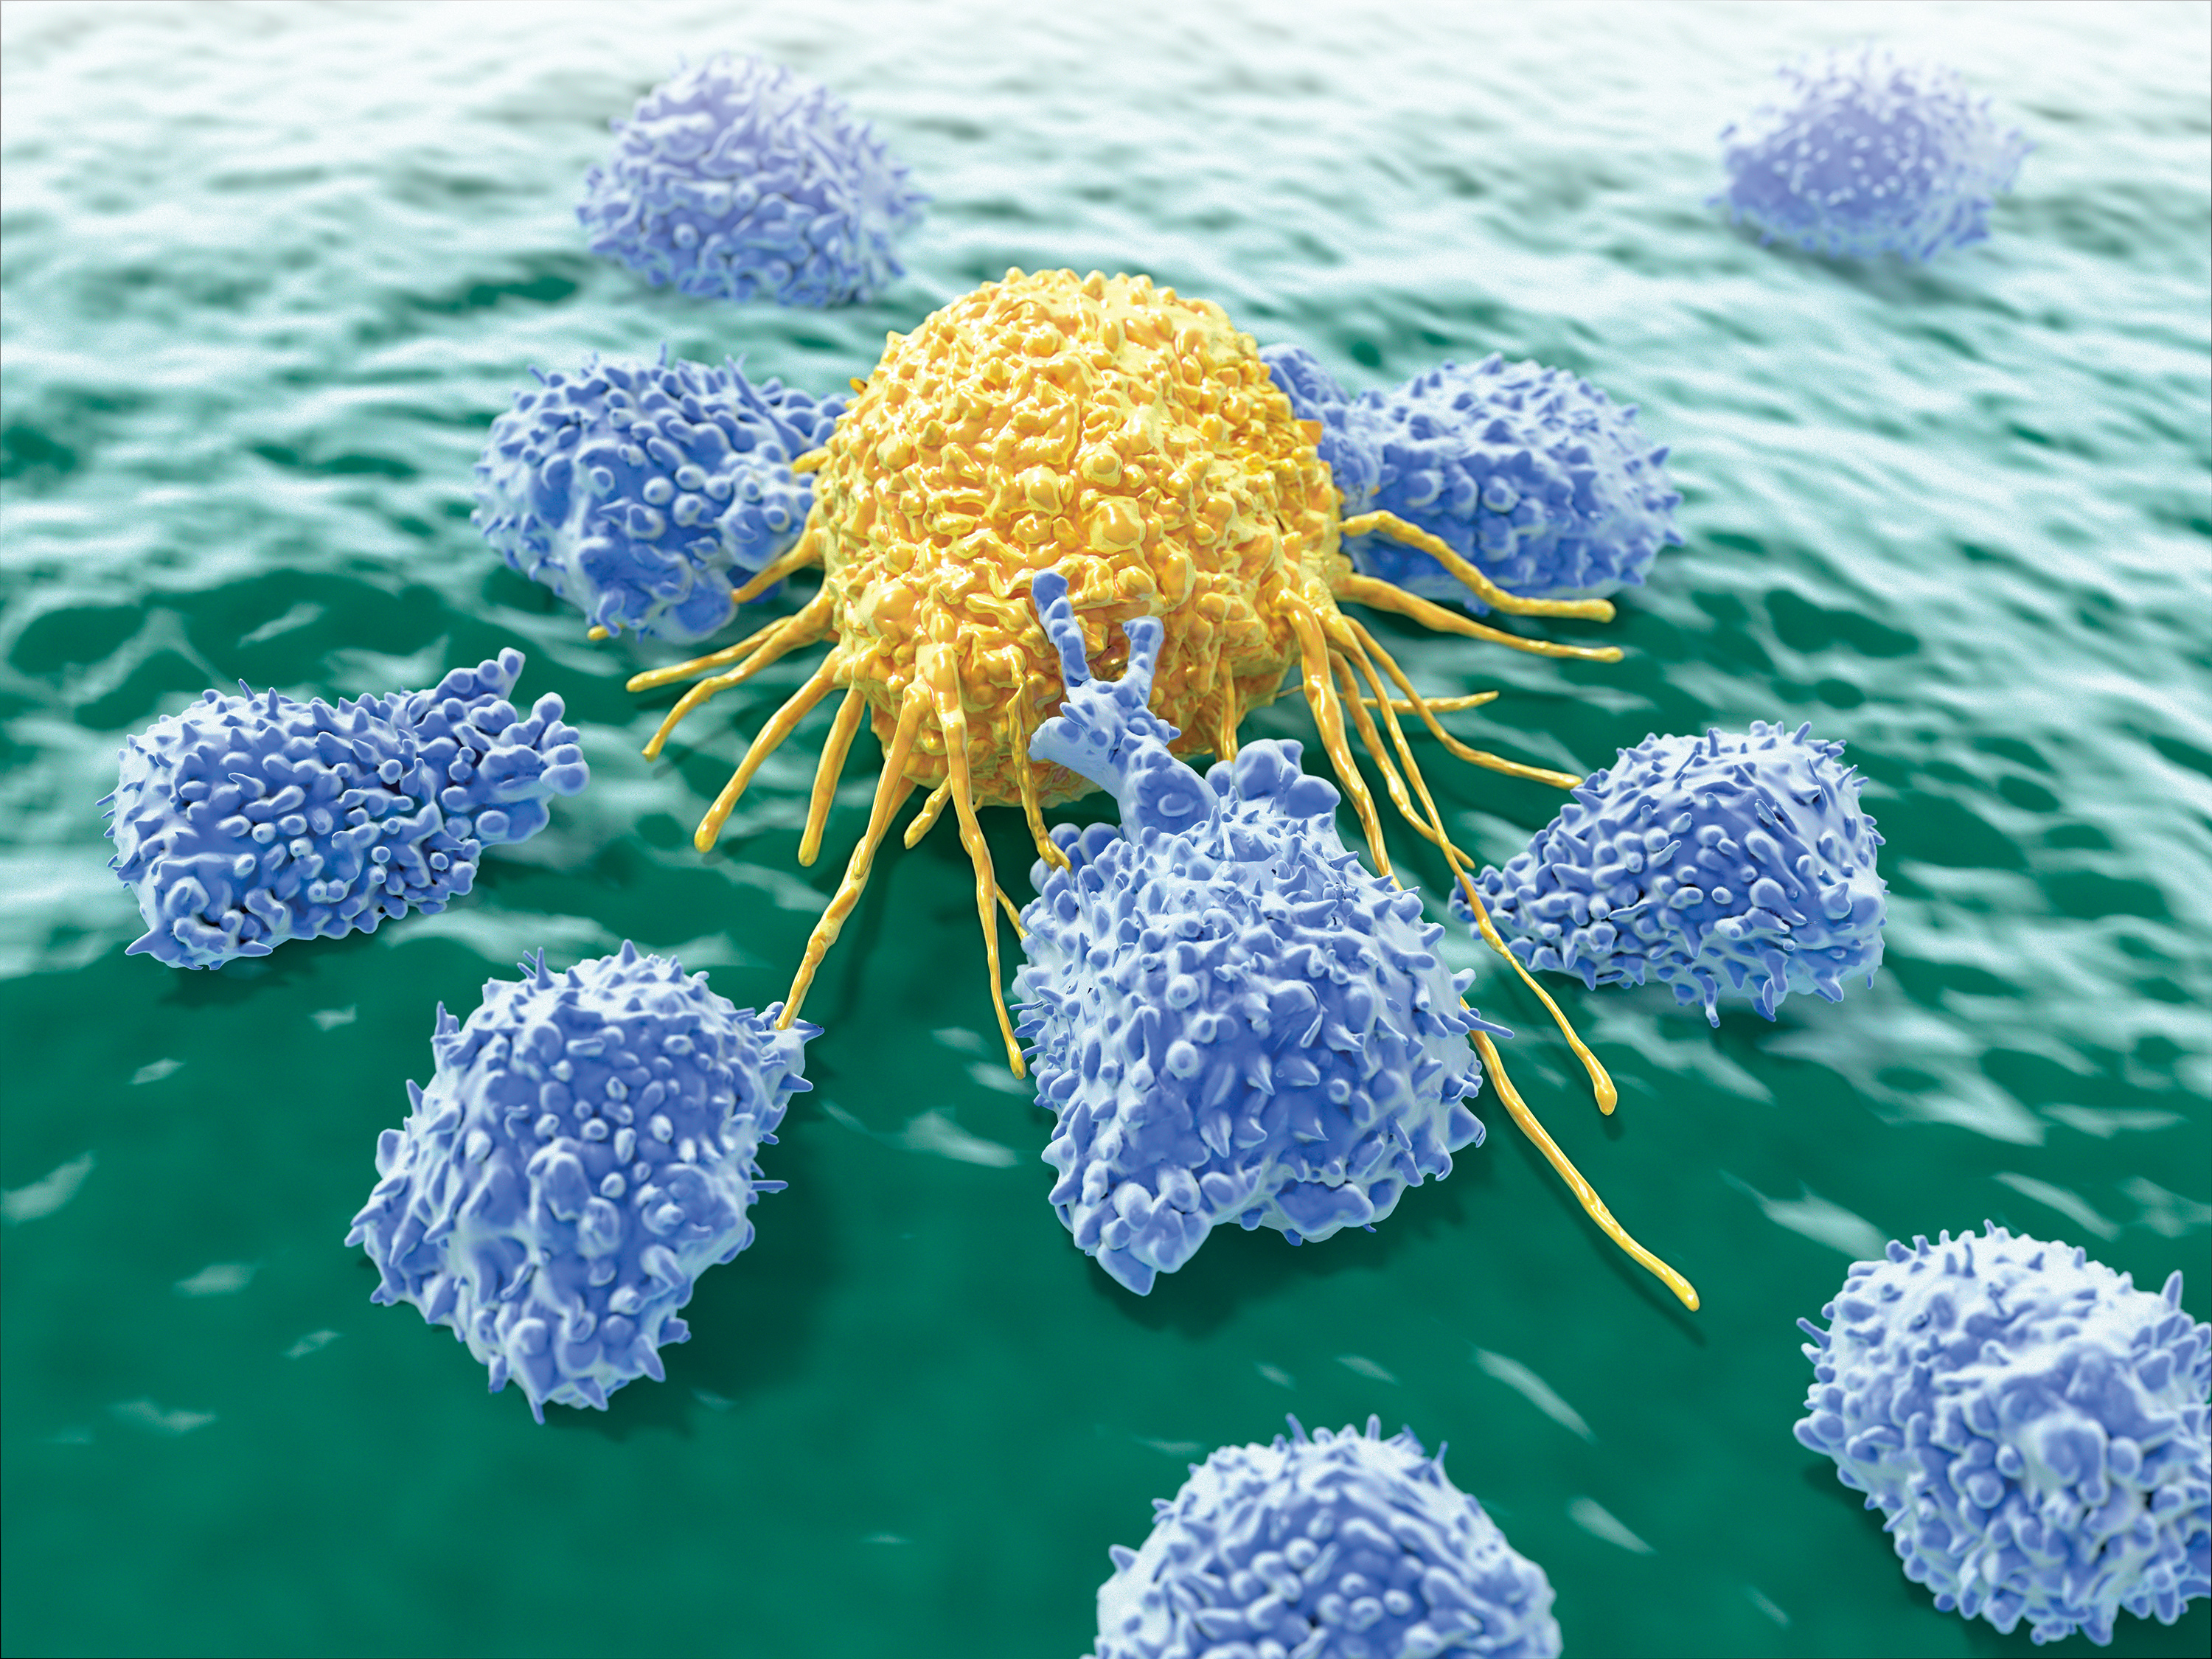
\includegraphics[width=\textwidth]{../Images/nk_cell_meb.jpg}
                \caption{Natural killer cells and a tumor cell}
            \end{figure}  
        \end{minipage}\hfill
        \begin{minipage}{0.6\textwidth}
            \begin{figure}
                \centering
                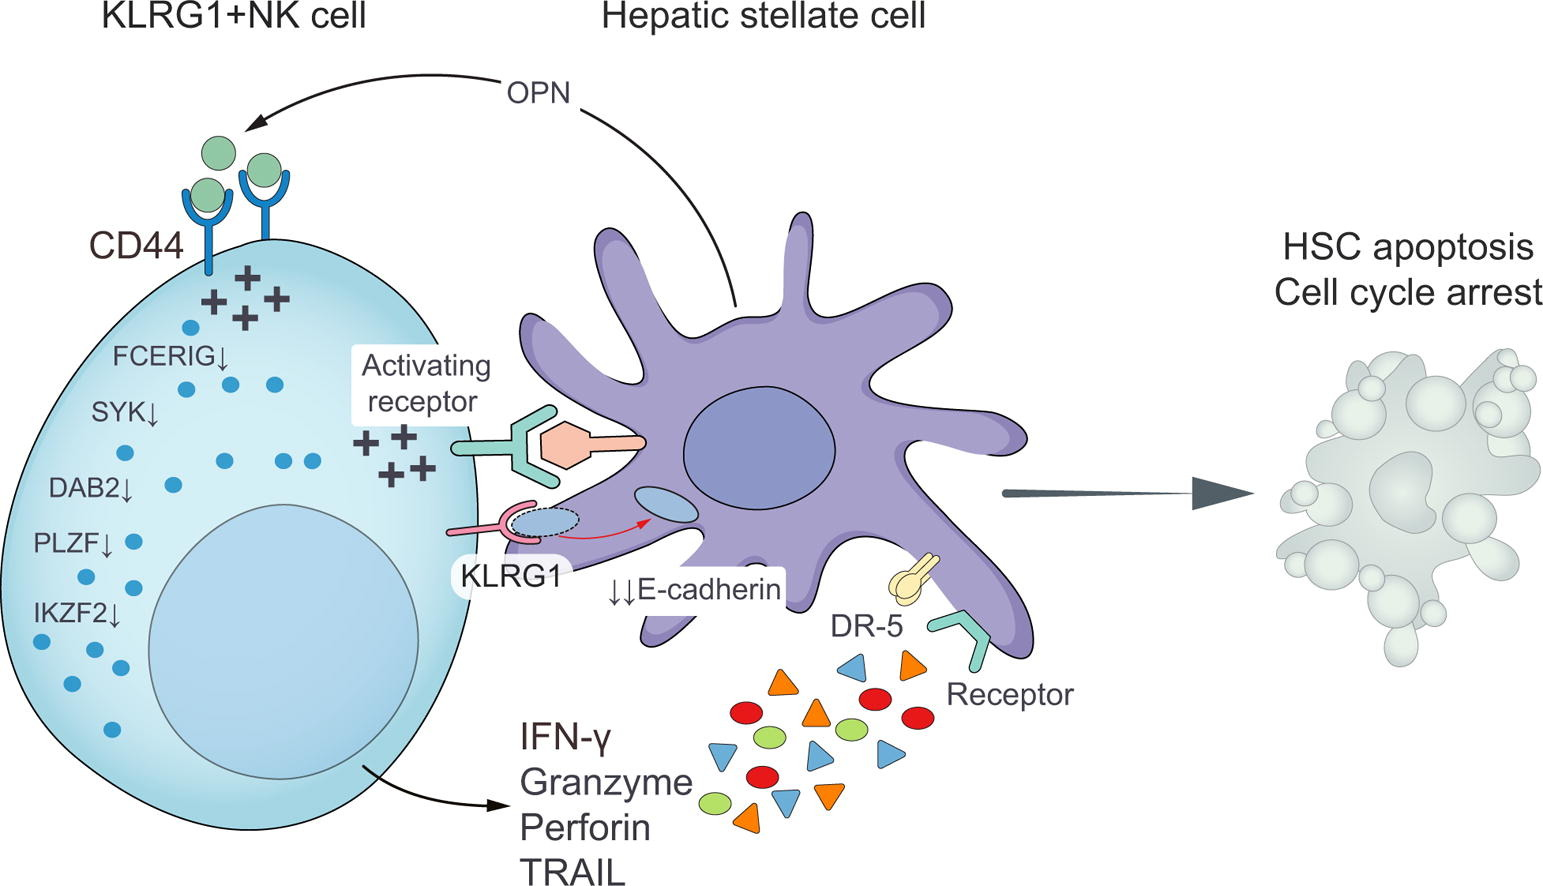
\includegraphics[width=\textwidth]{../Images/nk_cell_schematics.jpg}
                \caption{NK cell action mechanism}
            \end{figure}    
        \end{minipage}
    \end{block}
\end{frame}

\begin{frame}{Mechanisms of action of a monoclonal antibody}
    \begin{block}{Complement Dependent Cell Cytotoxicity}
        \begin{figure}
            \centering
            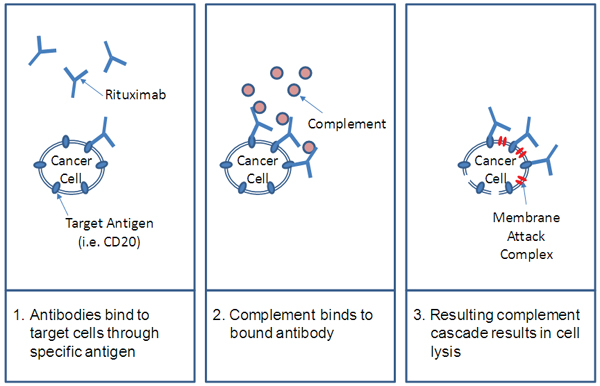
\includegraphics[width=0.8\textwidth]{../Images/complement-dependent-cellular-cytotoxicity.jpg}
            \caption{Tumor cell lysis induced \emph{via} antibody recognition}
            \label{fig:CDCC}
        \end{figure}
    \end{block}
\end{frame}

\begin{frame}{Mechanisms of action of a monoclonal antibody}
    \begin{block}{Summary of cell toxicity mechanisms}
        \begin{figure}
            \centering
            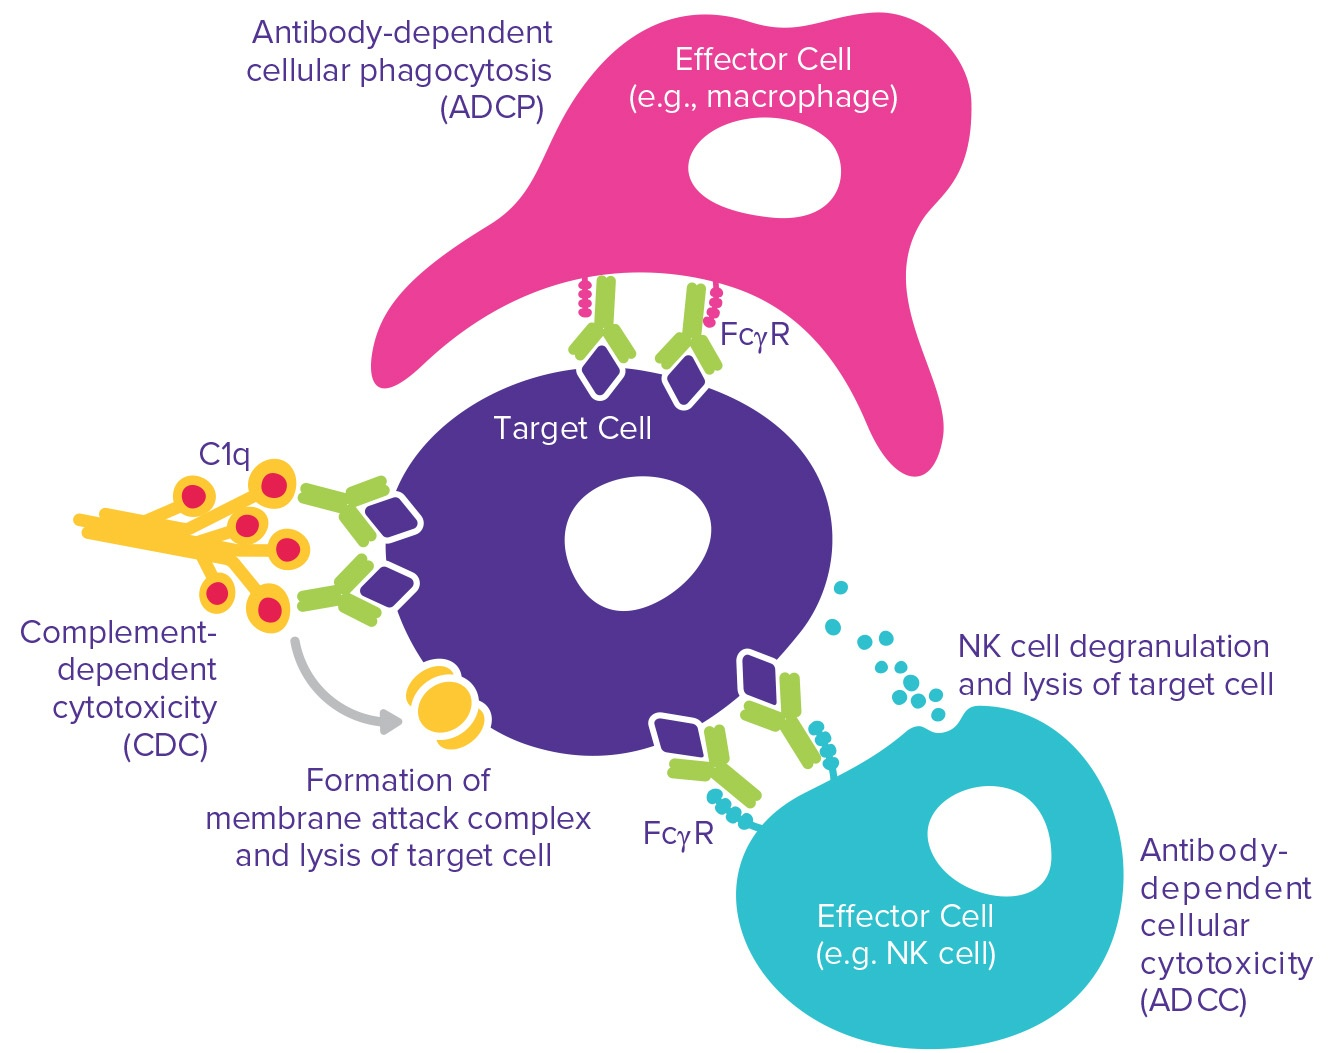
\includegraphics[width=0.8\textwidth]{../Images/recap_toxicity.jpg}
            % \caption{Tumor cell lysis induced \emph{via} antibody recognition}
            \label{fig:summary}
        \end{figure}
    \end{block}
\end{frame}